\section{\module{riutil} ---
         RenderMan utilities}

\declaremodule{extension}{cgkit.riutil}
\modulesynopsis{RenderMan utility functions}

\begin{funcdesc}{RiuArrow}{height=1.0, thickness=0.1, headheight=0.2, headscale=1.7}
\end{funcdesc}

\begin{funcdesc}{RiuCoordSystem}{thickness=0.06, shader="matte"}
\end{funcdesc}

\begin{funcdesc}{RiuDefaultHeader}{}
Outputs a default header into the RIB stream. This function can be
called right after \function{RiBegin()} to write the following
information into the RIB stream:

\begin{verbatim}
##RenderMan RIB-Structure 1.1
##Creator <Filename>
##CreationDate <Date>
##For <User>
\end{verbatim}

The "For" information is left out if the user name cannot be determined.
\end{funcdesc}

\begin{funcdesc}{RiuGrid}{thickness=0.02, cells=6, shader="matte", color=(0.9, 0.9, 0.9)}
Outputs a grid primitive. \var{thickness} determines the thickness of the
grid lines and \var{cells} the number of gridlines. The grid lies on the XY
plane and is centered at the origin. The grid spacing is 1 unit. The
grid uses the given shader and color.

\begin{center}
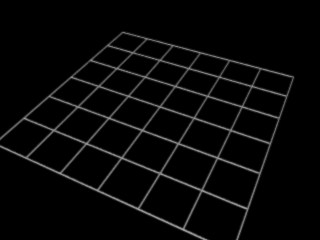
\includegraphics[width=6cm]{pics/grid}
\end{center}
\end{funcdesc}
